
%\usetikzlibrary{shapes,shapes.geometric,patterns} 

\begin{figure}

\centering
%%%%%%%%%%%%%%%%%%%%%%%%%%%  Confidentiality   %%%%%%%%%%%%%%%%%%%%%%%%%%%%%%%
\begin{subfigure}[b]{0.30\linewidth}
\centering
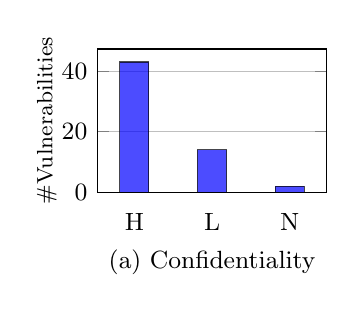
\begin{tikzpicture}
        \begin{axis}[
        width =4.5cm,
        height = 3.4cm,
        major x tick style = transparent,
        ybar=\pgflinewidth,
        bar width=10.5pt,
        ymajorgrids = true,
        xlabel = {(a) Confidentiality},
        ylabel = {{\footnotesize \#Vulnerabilities}}, 
        ylabel style={yshift=-5pt},
        symbolic x coords={H, L, N},
        xtick = data,
        scaled y ticks = false,
        enlarge x limits=0.24,
        ymin=0,
        legend style={at={(0.5,1.35)},
        cells={align=center},
        anchor=north,
        legend columns=4},
        font=\small
        ]
\addplot[style={black,fill=blue,mark=none},opacity=0.7]coordinates {(H, 43) (L, 14) (N, 2) };
%
%
%
%\addlegendentry{Overall}
%
\end{axis}
\end{tikzpicture}
\label{fig:confidentiality_overall}
\end{subfigure}
\hfill  %%%%%%%%%%%%%%%%%%%%%%%%% Integrity %%%%%%%%%%%%%%%%%%%%%%%%%%%%
\begin{subfigure}[b]{0.25\linewidth}
\centering
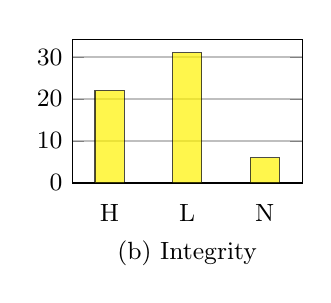
\begin{tikzpicture}
        \begin{axis}[
        width =4.5cm,
        height = 3.4cm,
        major x tick style = transparent,
        ybar=\pgflinewidth,
        bar width=10.5pt,
        ymajorgrids = true,
        xlabel = {(b) Integrity},
        %ylabel = {\#Vulnerabilities instances},
        symbolic x coords={H, L, N},
        xtick = data,
        scaled y ticks = false,
        enlarge x limits=0.24,
        ymin=0,
        legend style={at={(0.5,1.35)},
        cells={align=center},
        anchor=north,
        legend columns=4},
        font=\small
        ]
\addplot[style={black,fill=yellow,mark=none},opacity=0.7]coordinates {(H, 22) (L, 31) (N, 6) };
%
%
%
%\addlegendentry{Overall}
%
\end{axis}
\end{tikzpicture}
%\caption{Integrity}
\label{fig:integrity_overall}
\end{subfigure}
\hfill %%%%%%%%%%%%%%%%%%%%%%%%%%% Availability %%%%%%%%%%%%%%%%%%%%%%%%%%%%%%%
%\hspace{-20mm}
\begin{subfigure}[b]{0.27\linewidth}
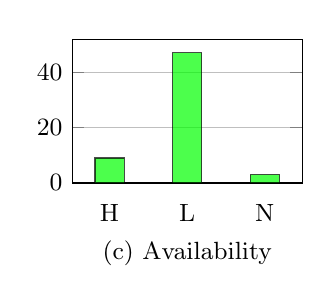
\begin{tikzpicture}
        \begin{axis}[
        width =4.5cm,
        height = 3.4cm,
        major x tick style = transparent,
        ybar=\pgflinewidth,
        bar width=10.5pt,
        ymajorgrids = true,
        xlabel = {(c) Availability},
        %ylabel = {\#Vulnerabilities instances},
        symbolic x coords={H, L, N},
        xtick = data,
        scaled y ticks = false,
        enlarge x limits=0.24,
        ymin=0,
        legend style={at={(0.5,1.35)},
        cells={align=center},
        anchor=north,
        legend columns=4},
        font=\small
        ]
\addplot[style={black,fill=green,mark=none},opacity=0.7]coordinates {(H, 9) (L, 47) (N, 3) };
%
%
%
%\addlegendentry{Overall}
%
\end{axis}
\end{tikzpicture}
\label{fig:availability_overall}
\end{subfigure}
\hfill  %%%%%%%%%%%%%%%%%%%%%%%%% Attack vector %%%%%%%%%%%%%%%%%%%%%%%%%%%%%%%
\begin{subfigure}[b]{0.30\linewidth}
\centering
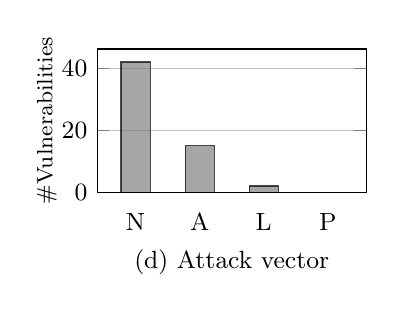
\begin{tikzpicture}
        \begin{axis}[
        width =5cm,
        height = 3.4cm,
        major x tick style = transparent,
        ybar=\pgflinewidth,
        bar width=10.5pt,
        ymajorgrids = true,
        xlabel = {(d) Attack vector},
        ylabel = {{\footnotesize \#Vulnerabilities }},
        ylabel style={yshift=-5pt},
        symbolic x coords={N, A, L,P},
        xtick = data,
        scaled y ticks = false,
        enlarge x limits=0.20,
        ymin=0,
        legend style={at={(0.5,1.35)},
        cells={align=center},
        anchor=north,
        legend columns=4},
        font=\small
        ]
\addplot[style={black,fill=gray,mark=none},opacity=0.7]coordinates {(N, 42) (A, 15) (L, 2) (P, 0) };
%\addlegendentry{Overall}
%
%
%
%
\end{axis}
\end{tikzpicture}
%\caption{Attack vector}
\label{fig:attack_vector_overall}
\end{subfigure}
\hfill %%%%%%%%%%%%%%%%%%%%%%%%%%%   Attack Complexity %%%%%%%%%%%%%%%%%%%%%%%%%%%%%%%
\hspace{10mm}
\begin{subfigure}[b]{0.25\linewidth}
\centering
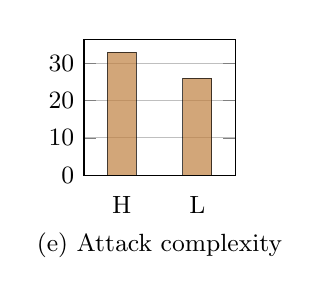
\begin{tikzpicture}
        \begin{axis}[
        width =3.5cm,
        height = 3.3cm,
        major x tick style = transparent,
        ybar=\pgflinewidth,
        bar width=10.5pt,
        ymajorgrids = true,
        xlabel = {(e) Attack complexity},
        %ylabel = {\#Vulnerabilities instances},
        symbolic x coords={H, L},
        xtick = data,
        scaled y ticks = false,
        enlarge x limits=0.50,
        ymin=0,
        legend style={at={(0.5,1.35)},
        cells={align=center},
        anchor=north,
        legend columns=4},
        font=\small
        ]
\addplot[style={black,fill=brown,mark=none},opacity=0.7]coordinates {(H, 33) (L, 26) };
%
%
%
%\addlegendentry{Overall}
%
\end{axis}
\end{tikzpicture}
%\caption{Attack Ccomplexity}
\label{fig:attack_complexity_overall}
\end{subfigure}
\hfill %%%%%%%%%%%%%%%%%%%%%%%%%%%  Base severity %%%%%%%%%%%%%%%%%%%%%%%%%%%%%%%
%\hspace{10mm}
\begin{subfigure}[b]{0.30\linewidth}
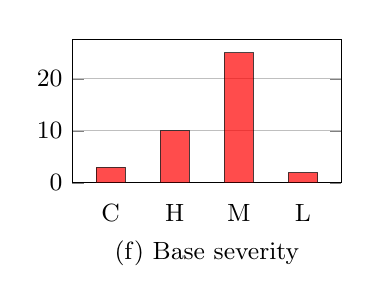
\begin{tikzpicture}
        \begin{axis}[
        width =5cm,
        height = 3.4cm,
        major x tick style = transparent,
        ybar=\pgflinewidth,
        bar width=10.5pt,
        ymajorgrids = true,
        xlabel = {(f) Base severity},
        %ylabel = {\#Vulnerabilities instances},
        symbolic x coords={C, H, M, L},
        xtick = data,
        scaled y ticks = false,
        enlarge x limits=0.20,
        ymin=0,
        legend style={at={(0.5,1.35)},
        cells={align=center},
        anchor=north,
        legend columns=4},
        font=\small
        ]
\addplot[style={black,fill=red,mark=none},opacity=0.7]coordinates {(C, 3) (H, 10) (M, 25) (L, 2) };
%\addlegendentry{Overall}
%
%
%
%
\end{axis}
\end{tikzpicture}
%\caption{Base severity}
\label{fig:base_severity_overall}
\end{subfigure}
\hspace{3.5mm}

\caption{Impact, exploitability and  severity   of   update traffic vulnerabilities: (a,b,c,e,f)=H:High, M:Medium, L:Low,  N:None, C:Critical. (d)=N:Network, A:Adjacent network, L:Local, P:Physical.}
\label{fig:update_traffic_impact}
\end{figure}

